\documentclass{article}
\usepackage[paper=letterpaper,margin=2cm]{geometry}
\usepackage[russian]{babel}
\usepackage[utf8]{inputenc}
\usepackage[]{graphicx}
\usepackage[usenames]{color}
\usepackage{colortbl}
\usepackage{geometry}
\usepackage{xcolor}
\usepackage{listings}
\usepackage{hyperref}

\geometry{
  a4paper,
  top=25mm, 
  right=30mm, 
  bottom=25mm, 
  left=30mm
}

\begin{document}

\begin{center}
  \section*{
    Федеральное государственное автономное образовательное учреждение\\ высшего образования\\
    «Национальный исследовательский университет ИТМО»\\
    Факультет Программной Инженерии и Компьютерной Техники \\
   }
  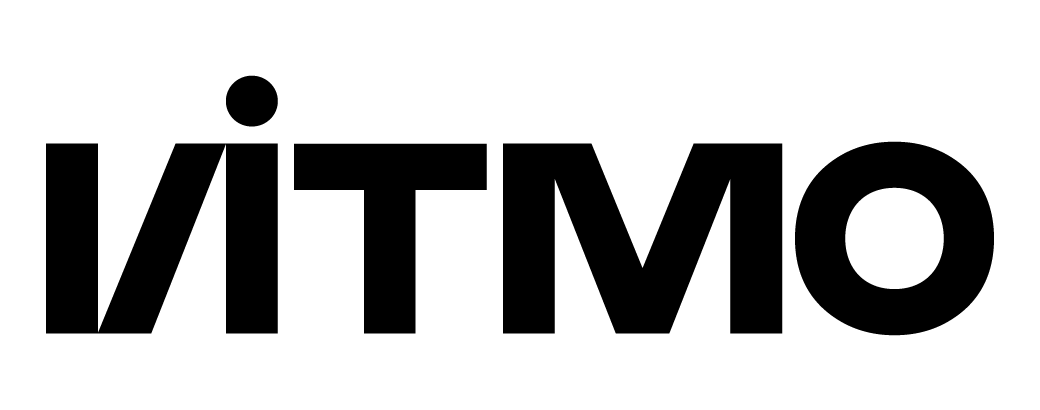
\includegraphics[scale=0.2]{../../lib/img/itmo.png}
\end{center}
\vspace{4cm}


\begin{center}
  \large \textbf{Вариант \textnumero 371364}\\
  \textbf{Лабораторная работа \textnumero 2}\\
  по дисциплине\\
  \textbf{Программирование}
\end{center}

\vspace*{\fill}

\begin{flushright}
  Выполнил Студент группы P3115\\
  \textbf{Владимир Мацюк}\\
  Преподаватель: \\
  \textbf{Сорокин Роман Борисович}\\
\end{flushright}

\vspace{1cm}

\begin{center}
  г. Санкт-Петербург\\
  2022г.
\end{center}

\newpage

\lstset{
  inputencoding=utf8,
  frame=single,
  language=Java,
  breaklines=true,
  numbers=left,
  postbreak=\mbox{\textcolor{red}{$\hookrightarrow$}\space},
  extendedchars=false,
  showspaces=false,
  showstringspaces=false,
  basicstyle=\footnotesize\ttfamily,
  identifierstyle=\bf\ttfamily\color[HTML]{2a72de},
  commentstyle=\color[rgb]{0.133,0.545,0.133},
  stringstyle=\color[rgb]{0.133,0.545,0.133},
  keywordstyle=\color[HTML]{5804cf}
}

\section*{Текст задания}

\begin{enumerate}
  \item Ознакомиться с документацией, обращая особое внимание на классы Pokemon и Move. При дальнейшем выполнении лабораторной работы читать документацию еще несколько раз.
  \itemСкачать файл Pokemon.jar. Его необходимо будет использовать как для компиляции, так и для запуска программы. Распаковывать его не надо! Нужно научиться подключать внешние jar-файлы к своей программе.
  \item Написать минимально работающую программу и посмотреть как она работает.
        \begin{lstlisting}
Battle b = new Battle();
Pokemon p1 = new Pokemon("Чужой", 1);
Pokemon p2 = new Pokemon("Хищник", 1);
b.addAlly(p1);
b.addFoe(p2);
b.go();
\end{lstlisting}
  \item Создать один из классов покемонов для своего варианта. Класс должен наследоваться от базового класса Pokemon. В конструкторе нужно будет задать типы покемона и его базовые характеристики. После этого попробуйте добавить покемона в сражение.
  \item Создать один из классов атак для своего варианта (лучше всего начать с физической или специальной атаки). Класс должен наследоваться от класса PhysicalMove или SpecialMove. В конструкторе нужно будет задать тип атаки, ее силу и точность. После этого добавить атаку покемону и проверить ее действие в сражении. Не забудьте переопределить метод describe, чтобы выводилось нужное сообщение.
  \item Если действие атаки отличается от стандартного, например, покемон не промахивается, либо атакующий покемон также получает повреждение, то в классе атаки нужно дополнительно переопределить соответствующие методы (см. документацию). При реализации атак, которые меняют статус покемона (наследники StatusMove), скорее всего придется разобраться с классом Effect. Он позволяет на один или несколько ходов изменить состояние покемона или модификатор его базовых характеристик.
  \item Доделать все необходимые атаки и всех покемонов, распределить покемонов по командам, запустить сражение.
\end{enumerate}

\section*{Ссылка на github}
\url{https://github.com/Wgmlgz/itmo/tree/main/prog/lab1}

\section*{Вывод}
Я ознакомолся с основами Java и изучил базовые инструманты для работы с ней.
\end{document}
